\section{Une histoire de température}

Solène et Nicolas ont tracé le graphique de l'évolution de la masse de de l'air enfermé dans une enceinte en fonction du volume disponible. Mais ils n'ont pas effectué leurs mesures à la même température.

\begin{center}
	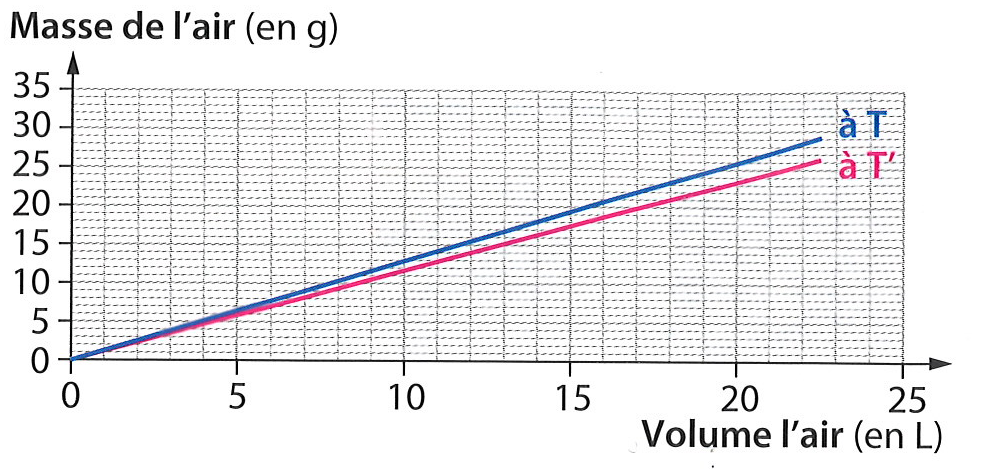
\includegraphics[scale=0.5]{masse}
\end{center}

\begin{questions}
	\question \`A la température $T'$, quelle est la masse d'air qui occupe un volume de 20 ml ?
	\fillwithdottedlines{2cm}
	
	\question Calculer la valeur de la masse volumique de l'air $\rho '_{air} $ à cette température $T'$ (rappel : $\rho = \dfrac{m}{V}$).
	\fillwithdottedlines{3cm}
	
	\question Relever la valeur de la masse d'air pour 20 ml  à la température $T$.
	
	\fillwithdottedlines{2cm}
	
	\question Calculer la valeur de $\rho_{air} $ à la température $T$.
	
	\fillwithdottedlines{3cm}
	
	
	\newpage
	
	\question Comparer $\rho_{air}$ et $\rho'_{air}$. En déduire quelle est la température la plus importante entre $T$ et $T'$.
	
	\fillwithdottedlines{4cm}
	
	
\end{questions}

